\section{CI/CD}

\subsection{Automated application deployment}

\subsubsection{Declaring deployment enviroments}

Environments in CI definitions describe where code gets deployed. It can be linked to a kubernetes cluster and usually 
defines a name and url for monitoring the overall application state.

Monitoring a deployment in GitLab requires installation and configuration of Prometheus.  

\subsubsection{Kubernetes application ressources}
Docker Image Tag can be built by combining GitLab variables: 

\ttfamily 
\$CI\_REGISTRY\_IMAGE:\$CI\_COMMIT\_SHORT\_SHA 
\rmfamily

To apply a kubernetes yaml manifest during CI/CD Pipeline, use the following script line:

\ttfamily
cat k8s.yaml | envsubst | kubectl apply -f -
\rmfamily

Inside the kubernetes yaml manifest, the image can be specified using a variable such as
``\$\{DOCKER\_IMAGE\_TAG\}'' 

\subsubsection{Deploying an application to Kubernetes}
Kubernetes Cluster needs to be configured as deployment destination in GitLab repository. 
For this, an agent must be installed inside the cluster. This agent can then be used to communicate through a NAT, access
cluster API endpoints in real time, push information about events as well as enable a cache of kubernetes objects.

With a GitOps workflow, kubernetes manifests are kept inside GitLab, and on every change to the repository manifests, 
the agent inside the cluster automatically updates resources accordingly. This is considered pull-based, because the cluster
agent actively pulls from the repository.   

The classical CI/CD workflow pushes new configuration from the GitLab repository to the claster using 
GitLab CI script commands on the kubernetes API.

Environment scope defines which environments are automatically assigned to this cluster when created.

\subsubsection{Deploying tokens and pulling secrets}
How does the kubernetes cluster access information inside our gitlab repository?
Creating a deploy token we can provide the kubernetes cluster with authentication credentials to pull images from the GitLab container registry.
read\_registry access should be enough.

These credentials must be saved as environment variables inside the 
GitLab repository and can then be used to create a kubernetes secret inside the CI script.
This kubernetes secret is used as ``ImagePullSecret'' inside the manifest to create resources.

\begin{figure}[h]
    \centering
    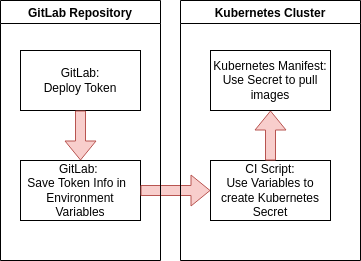
\includegraphics[width=6cm]{cicd-cluster-authentication.png}
    \caption{Cluster Authentication}
\end{figure}

\subsubsection{Dynamic environments and review apps}

Defining job environment variables inside the CI Script allows us to use the same k8s file for different branches, referencing different applications
\begin{itemize}
    \item DEPLOY\_SUFFIX
    \item DEPLOY\_HOST
\end{itemize}

\begin{figure}[h]
    \centering
    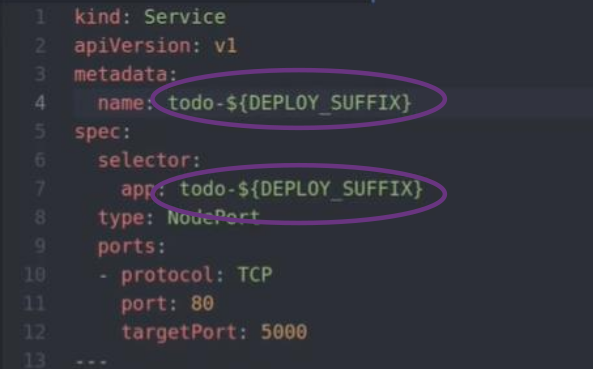
\includegraphics[width=8cm]{cicd-environment-variables.png}
    \caption{Using environment variables defined in CI-Job}
\end{figure}

Review Apps can be created automatically when pushing to any non-production branch. CI\_COMMIT\_REF\_SLUG creates a valid k8s name from the branch name. 
A new environment in GitLab is created automatically.

\begin{figure}[h]
    \centering
    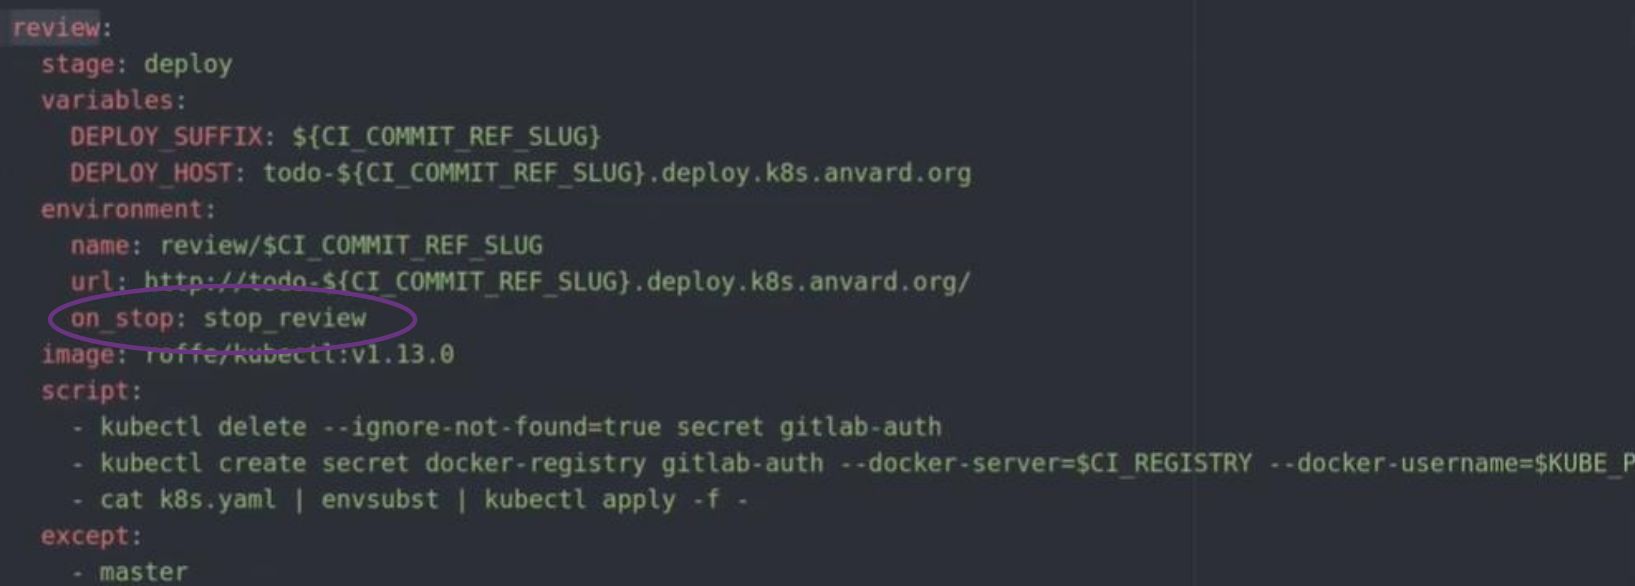
\includegraphics[width=\textwidth   ]{cicd-review-apps}
    \caption{Automatically creating review apps for branches}
\end{figure}

\subsection{Application Quality and Monitoring}
Integration and functional testing can be supported either using review apps or defining instances of containers as services. This makes the service available to the 
main container built inside the CI job.

\subsubsection{Analyzing code quality}
Separate jobs that check code quality inside the build pipeline provide results either as reports in merge requests or as separate job artifacts.
Code Quality jobs usually run parallel with the other test jobs to reduce overall pipeline time. 

Gitlab provides an image specifically for code quality which creates JSON reports -- comparing results to previous ones automatically is not a free feature in GitLab.

\subsubsection{Dynamic application security testing -- DAST}
Usually occurs after the deploy stage. Creates a JSON report and compares it with the last one to check for any differences to the reports from previous merges. Not a free feature.

\subsubsection{Application monitoring with Prometheus}



\subsection{Custom CI Infrastructure}

\subsubsection{Runners}